\documentclass[a4paper,14pt]{extarticle} 
\usepackage[a4paper,top=1.5cm, bottom=1.5cm, left=2cm, right=1cm]{geometry}
%\usepackage[T2A]{fontenc}
%\usepackage[english, russian]{babel}
\usepackage{graphicx}
\DeclareGraphicsExtensions{.pdf,.png,.jpg}

\usepackage{fontspec}
\setmainfont{Times New Roman}
\setsansfont{FreeSans}
\setmonofont{FreeMono}
\renewcommand{\baselinestretch}{1.5}
\usepackage{polyglossia}
\setdefaultlanguage{russian}
\setotherlanguages{english,russian}
\usepackage{setspace}
\usepackage[many]{tcolorbox}

\begin{document}
    \begin{center}
        \thispagestyle{empty}
        \begin{singlespace}
        ФЕДЕРАЛЬНОЕ АГЕНТСТВО СВЯЗИ

        ФЕДЕРАЛЬНОЕ ГОСУДАРСТВЕННОЕ БЮДЖЕТНОЕ ОБРАЗОВАТЕЛЬНОЕ

        УЧРЕЖДЕНИЕ ВЫСШЕГО ОБРАЗОВАНИЯ

        «САНКТ-ПЕТЕРБУРГСКИЙ ГОСУДАРСТВЕННЫЙ УНИВЕРСИТЕТ ТЕЛЕКОММУНИКАЦИЙ ИМ. ПРОФ. М.А. БОНЧ-БРУЕВИЧА»

        (СПбГУТ)
        \end{singlespace}
        \vspace{-1ex}
        \rule{\textwidth}{0.4pt}
        \vspace{-5ex}

        Факультет \underline{Инфокоммуникационных сетей и систем}

        Кафедра \underline{Защищенных систем связи}
        \vspace{10ex}

        \textbf{Лабораторная работа №1}\\
        Изучение протоколов сетевой аутентификации в сетях ОС Windows


    \end{center}
    \vspace{4ex}
    \begin{flushright}
    \parbox{10 cm}{
    \begin{flushleft}
        Выполнили студенты группы ИКТЗ-83:

        \underline{Громов А.А., Миколаени М.С.} \hfill \rule[-0.85ex]{0.1\textwidth}{0.6pt}

        \footnotesize \textit{ (Ф.И.О., № группы) \hfill (подпись)} \normalsize

        Проверил:

        \underline{Цветков А.Ю.} \hfill \rule[-0.85ex]{0.1\textwidth}{0.6pt}

        (\footnotesize \textit{уч. степень, уч. звание, Ф.И.О.) \hfill (подпись)} \normalsize

    \end{flushleft}
    }
    \end{flushright}
    \begin{center}
        \vfill
        Санкт-Петербург

        2020

    \end{center}
    \newpage

    \textbf{Цель лабораторной работы:}
    \vspace{-2em}
    \begin{enumerate}
        \begin{singlespace}
            \item Познакомиться с интерфейсом управления ролей Windows Server.
            \item Познакомиться со структурой контроллера домена.
            \item Изучить процесс аутентификации по протоколу NTLMv2 и Kerberos.   
        \end{singlespace}
    \end{enumerate}
    Схема сети:
    \begin{center}
        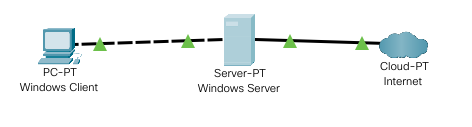
\includegraphics{pics/net.png}
    \end{center}
    \textbf{Пункт 9:} 
    \begin{center}
        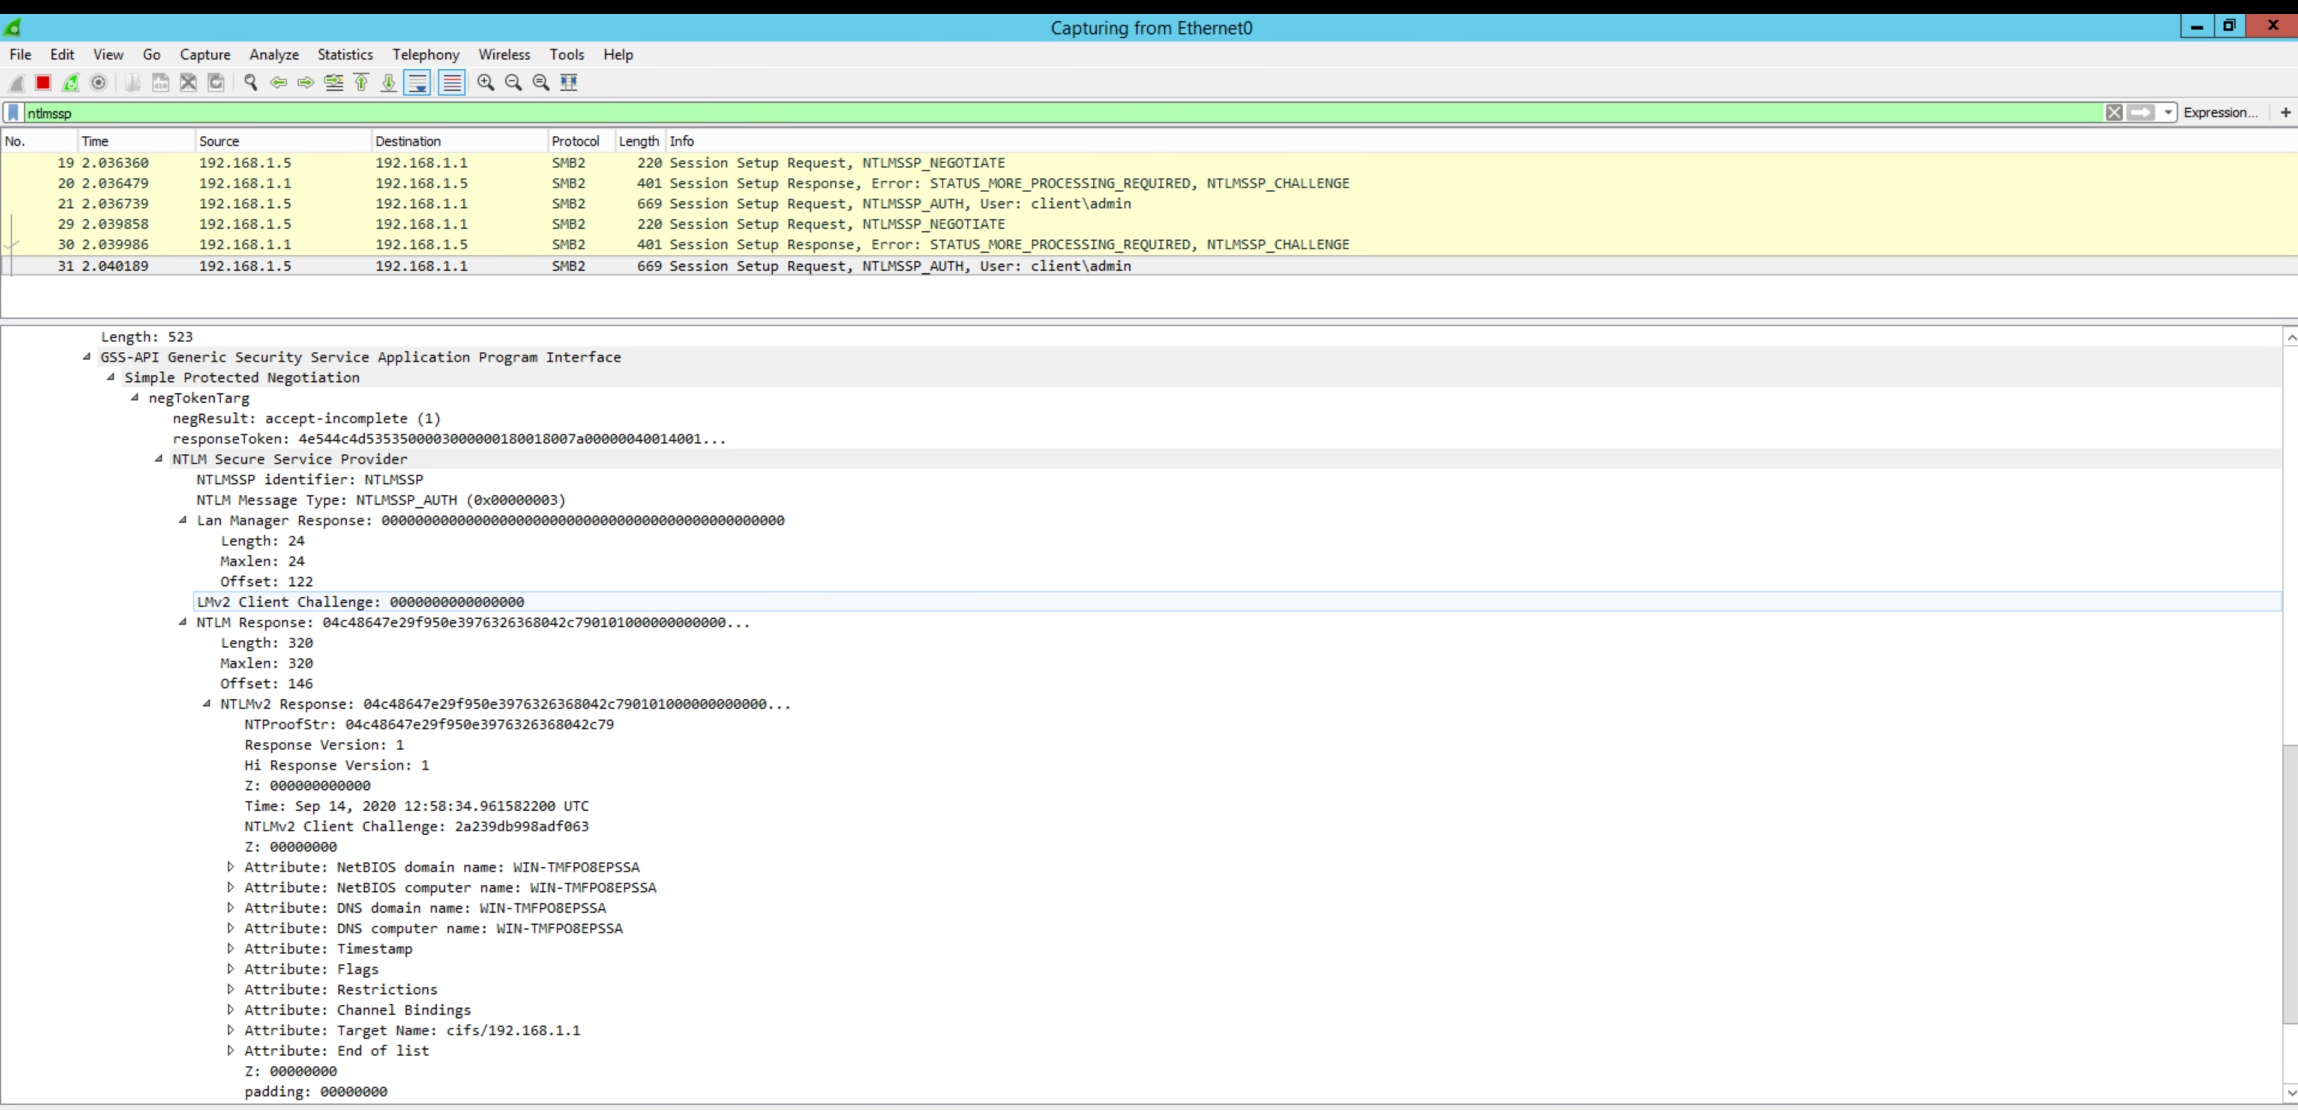
\includegraphics[scale=0.22]{pics/9.jpg}
    \end{center} 
    \newpage 
    \textbf{Пункт 24:}\\
    AS-REQ:
    \vspace{-2em}
    \begin{center}
        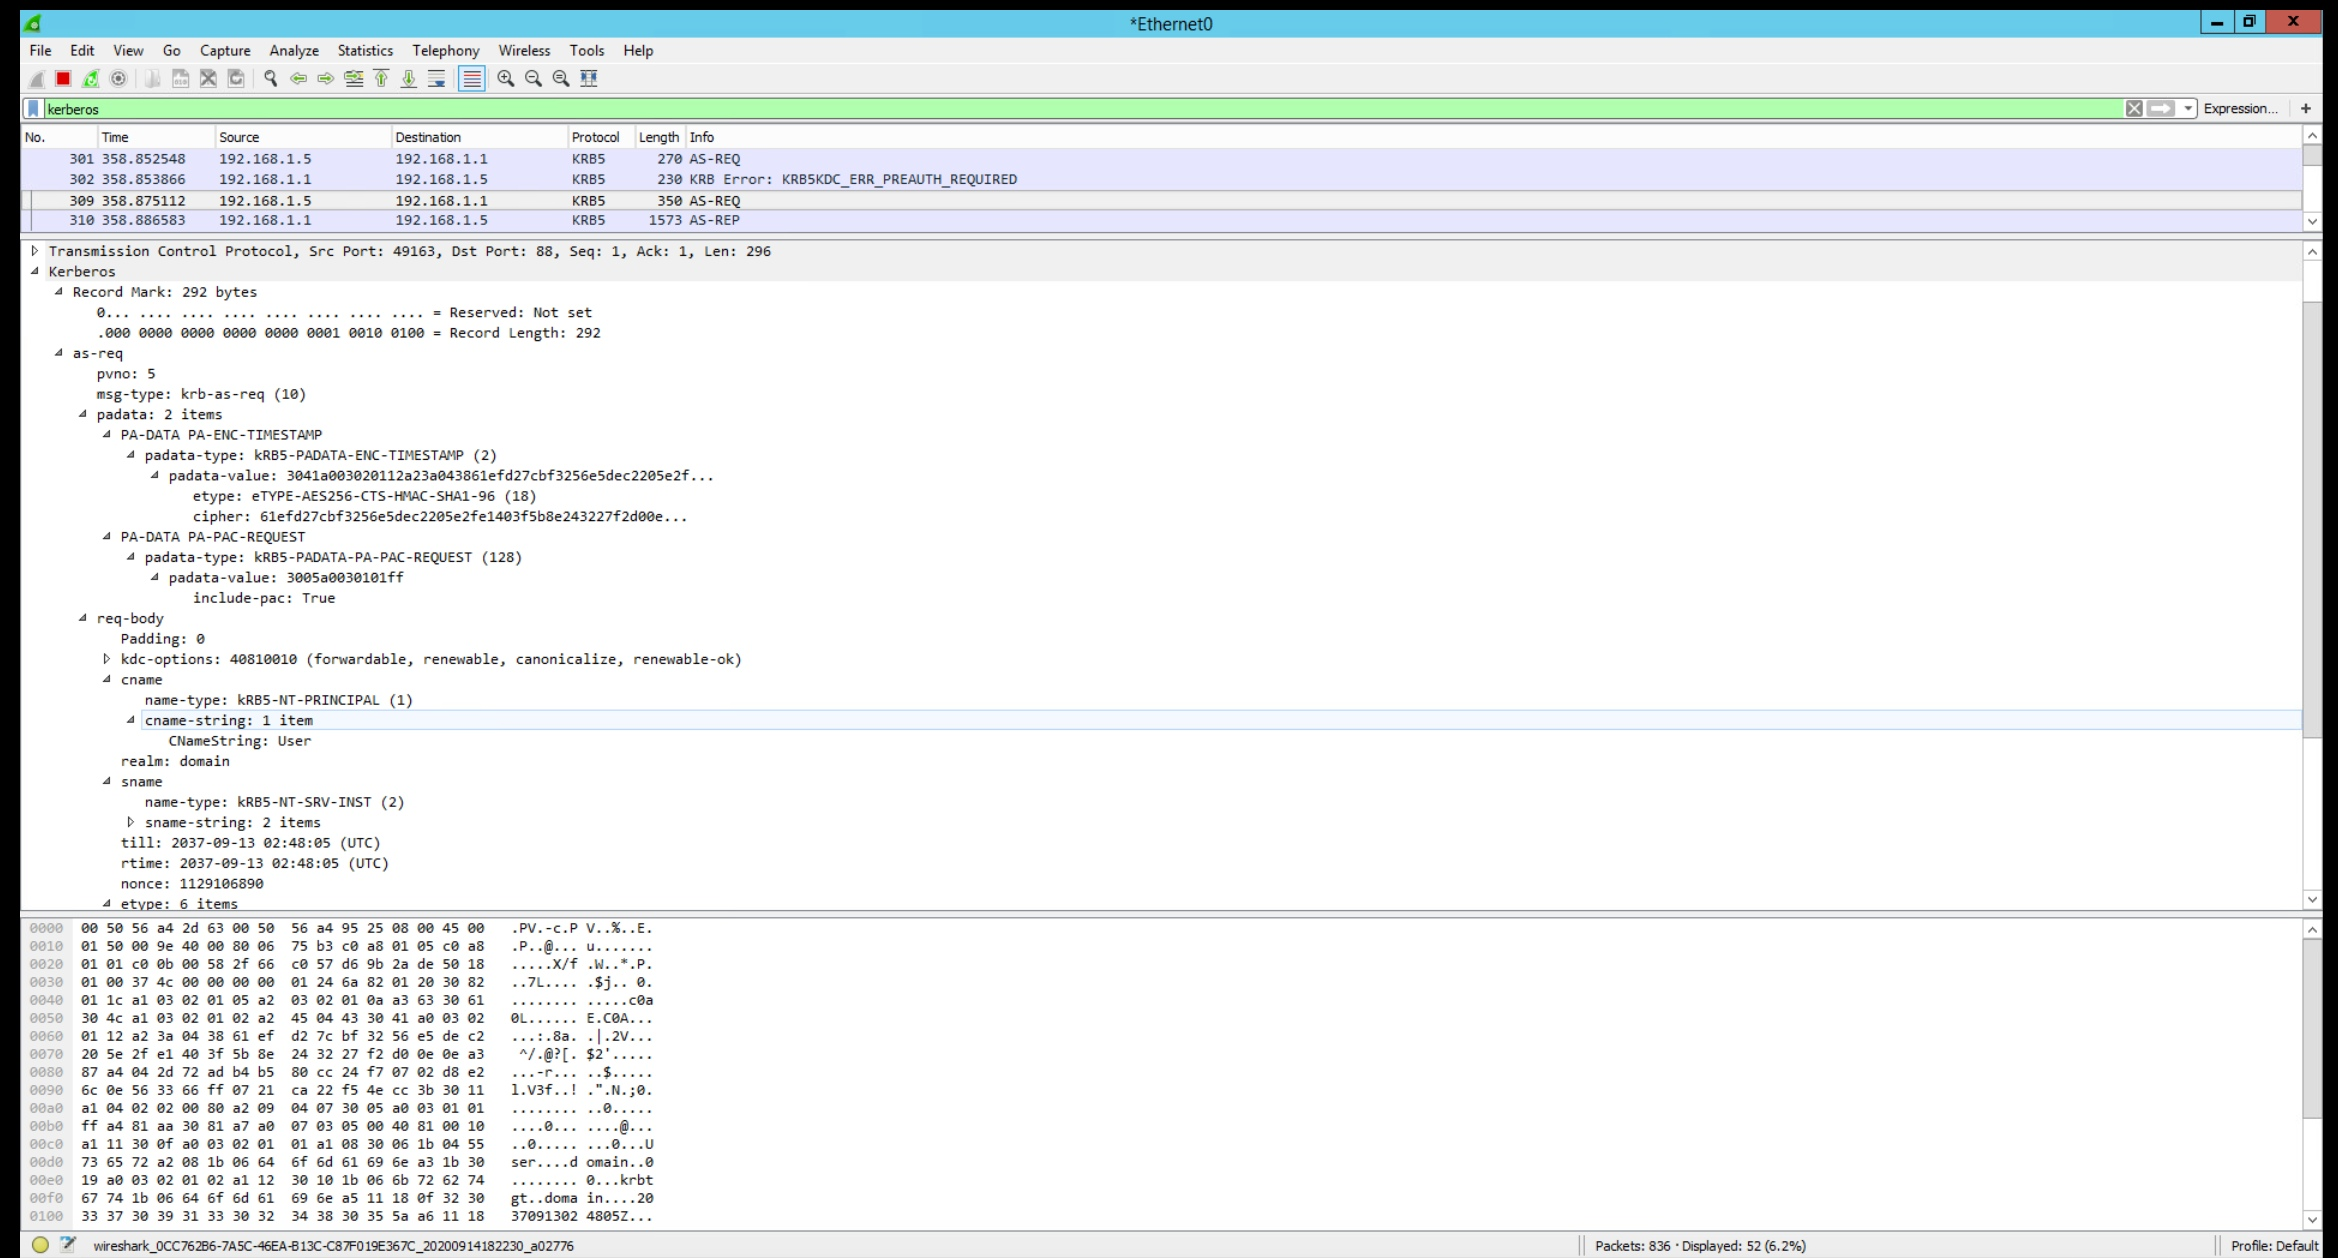
\includegraphics[scale=0.22]{pics/AS-REQ.jpg}
    \end{center}
    AS-REP:
    \vspace{-2em}
    \begin{center}
        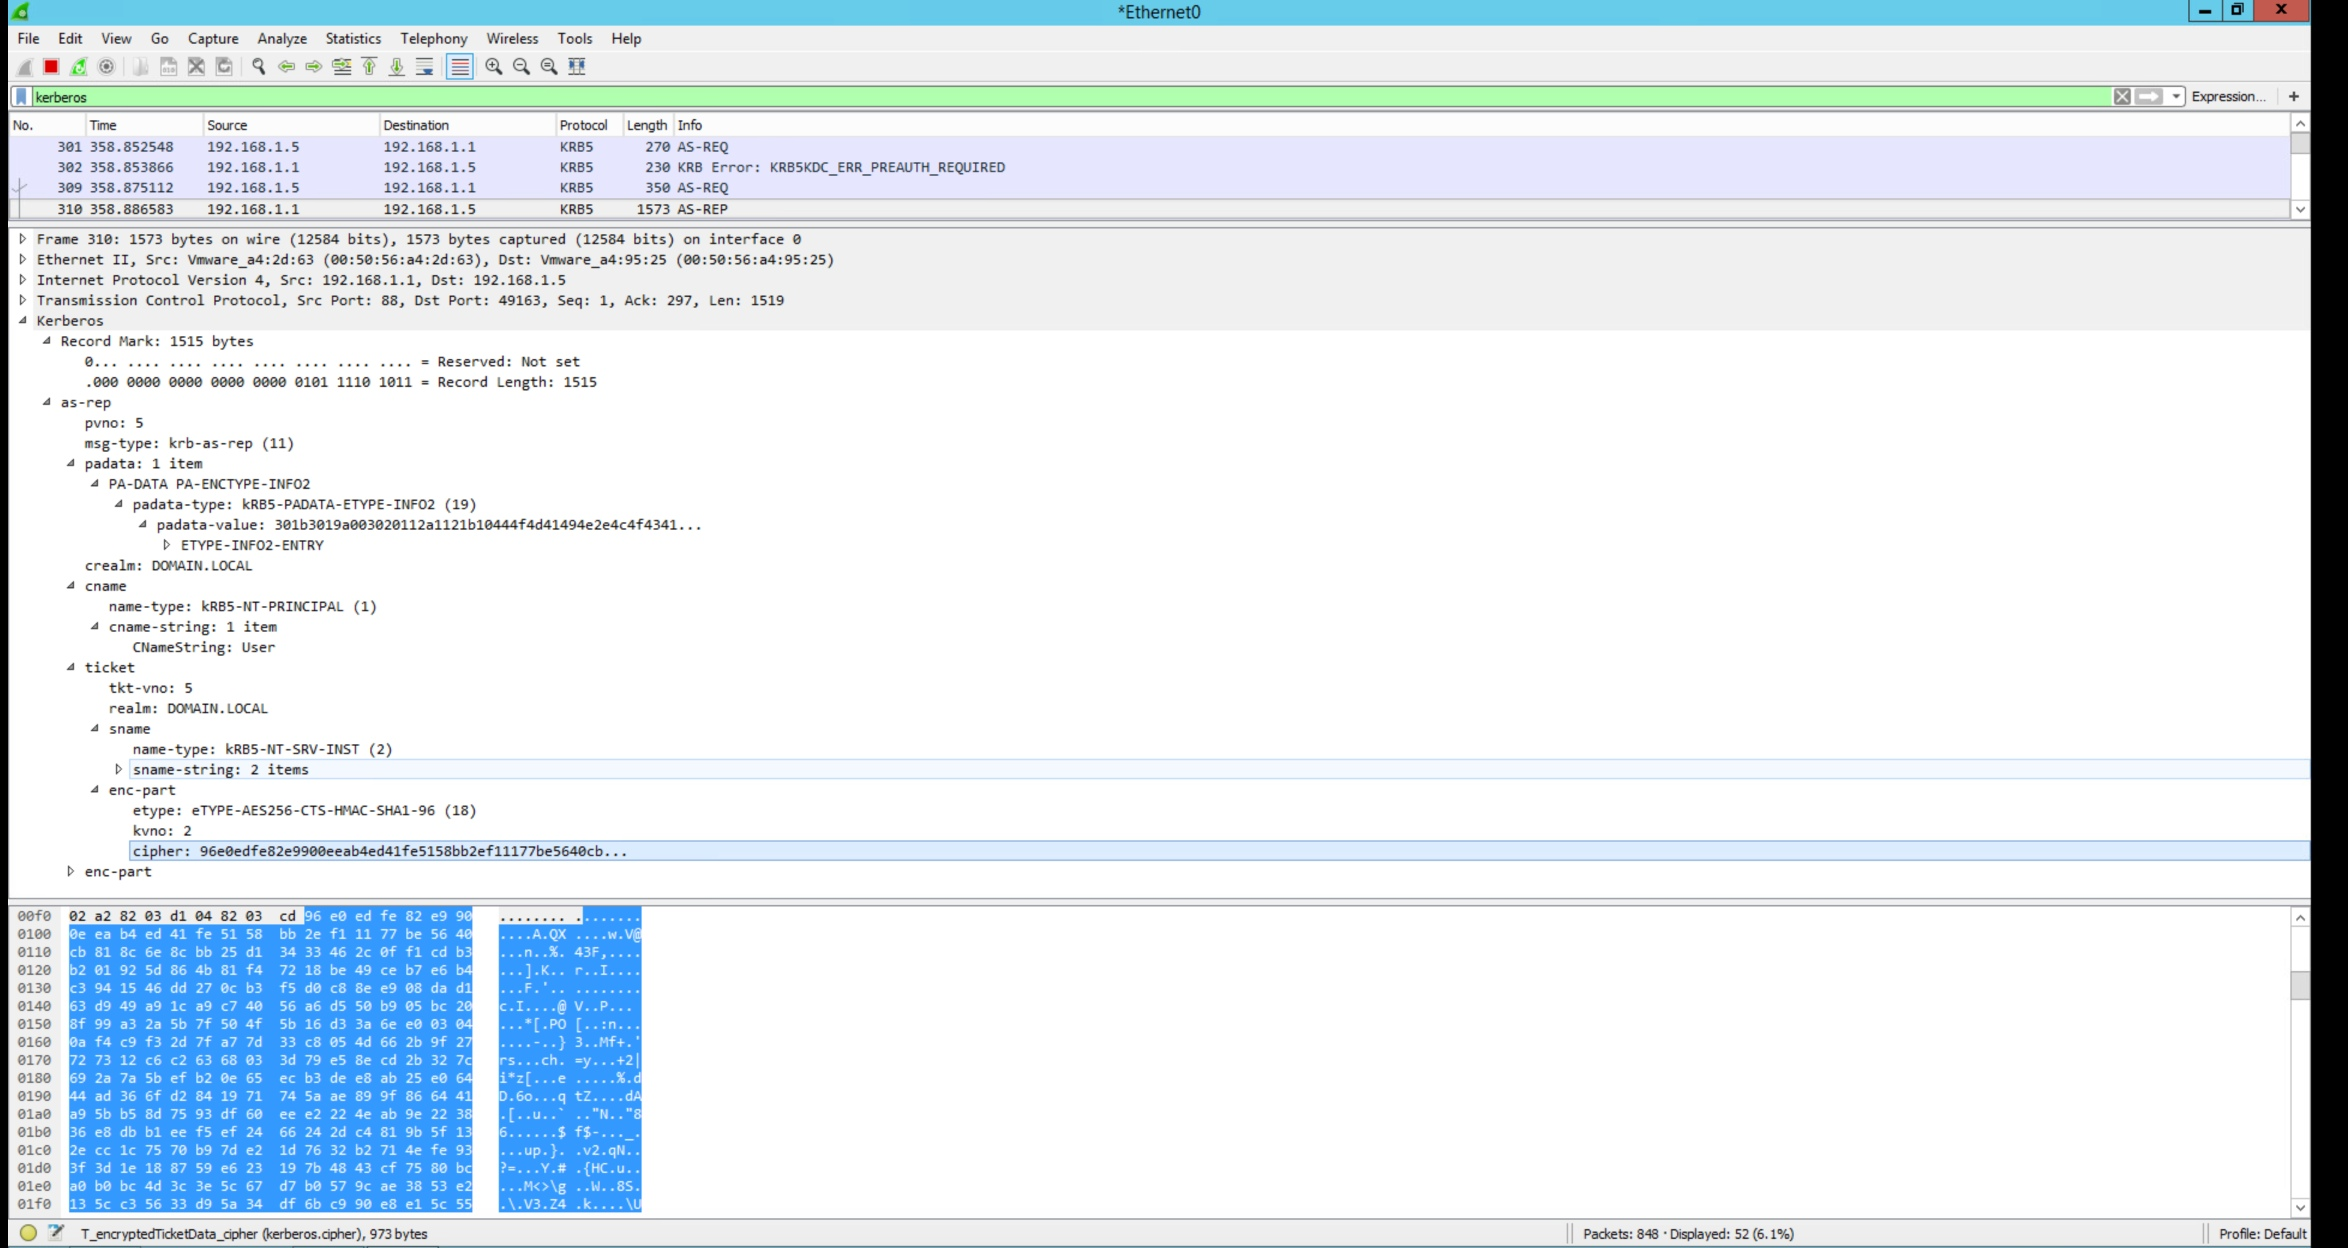
\includegraphics[scale=0.22]{pics/AS-REP.jpg}
    \end{center}
    \newpage
    \noindent TGS-REQ:
    \begin{center}
        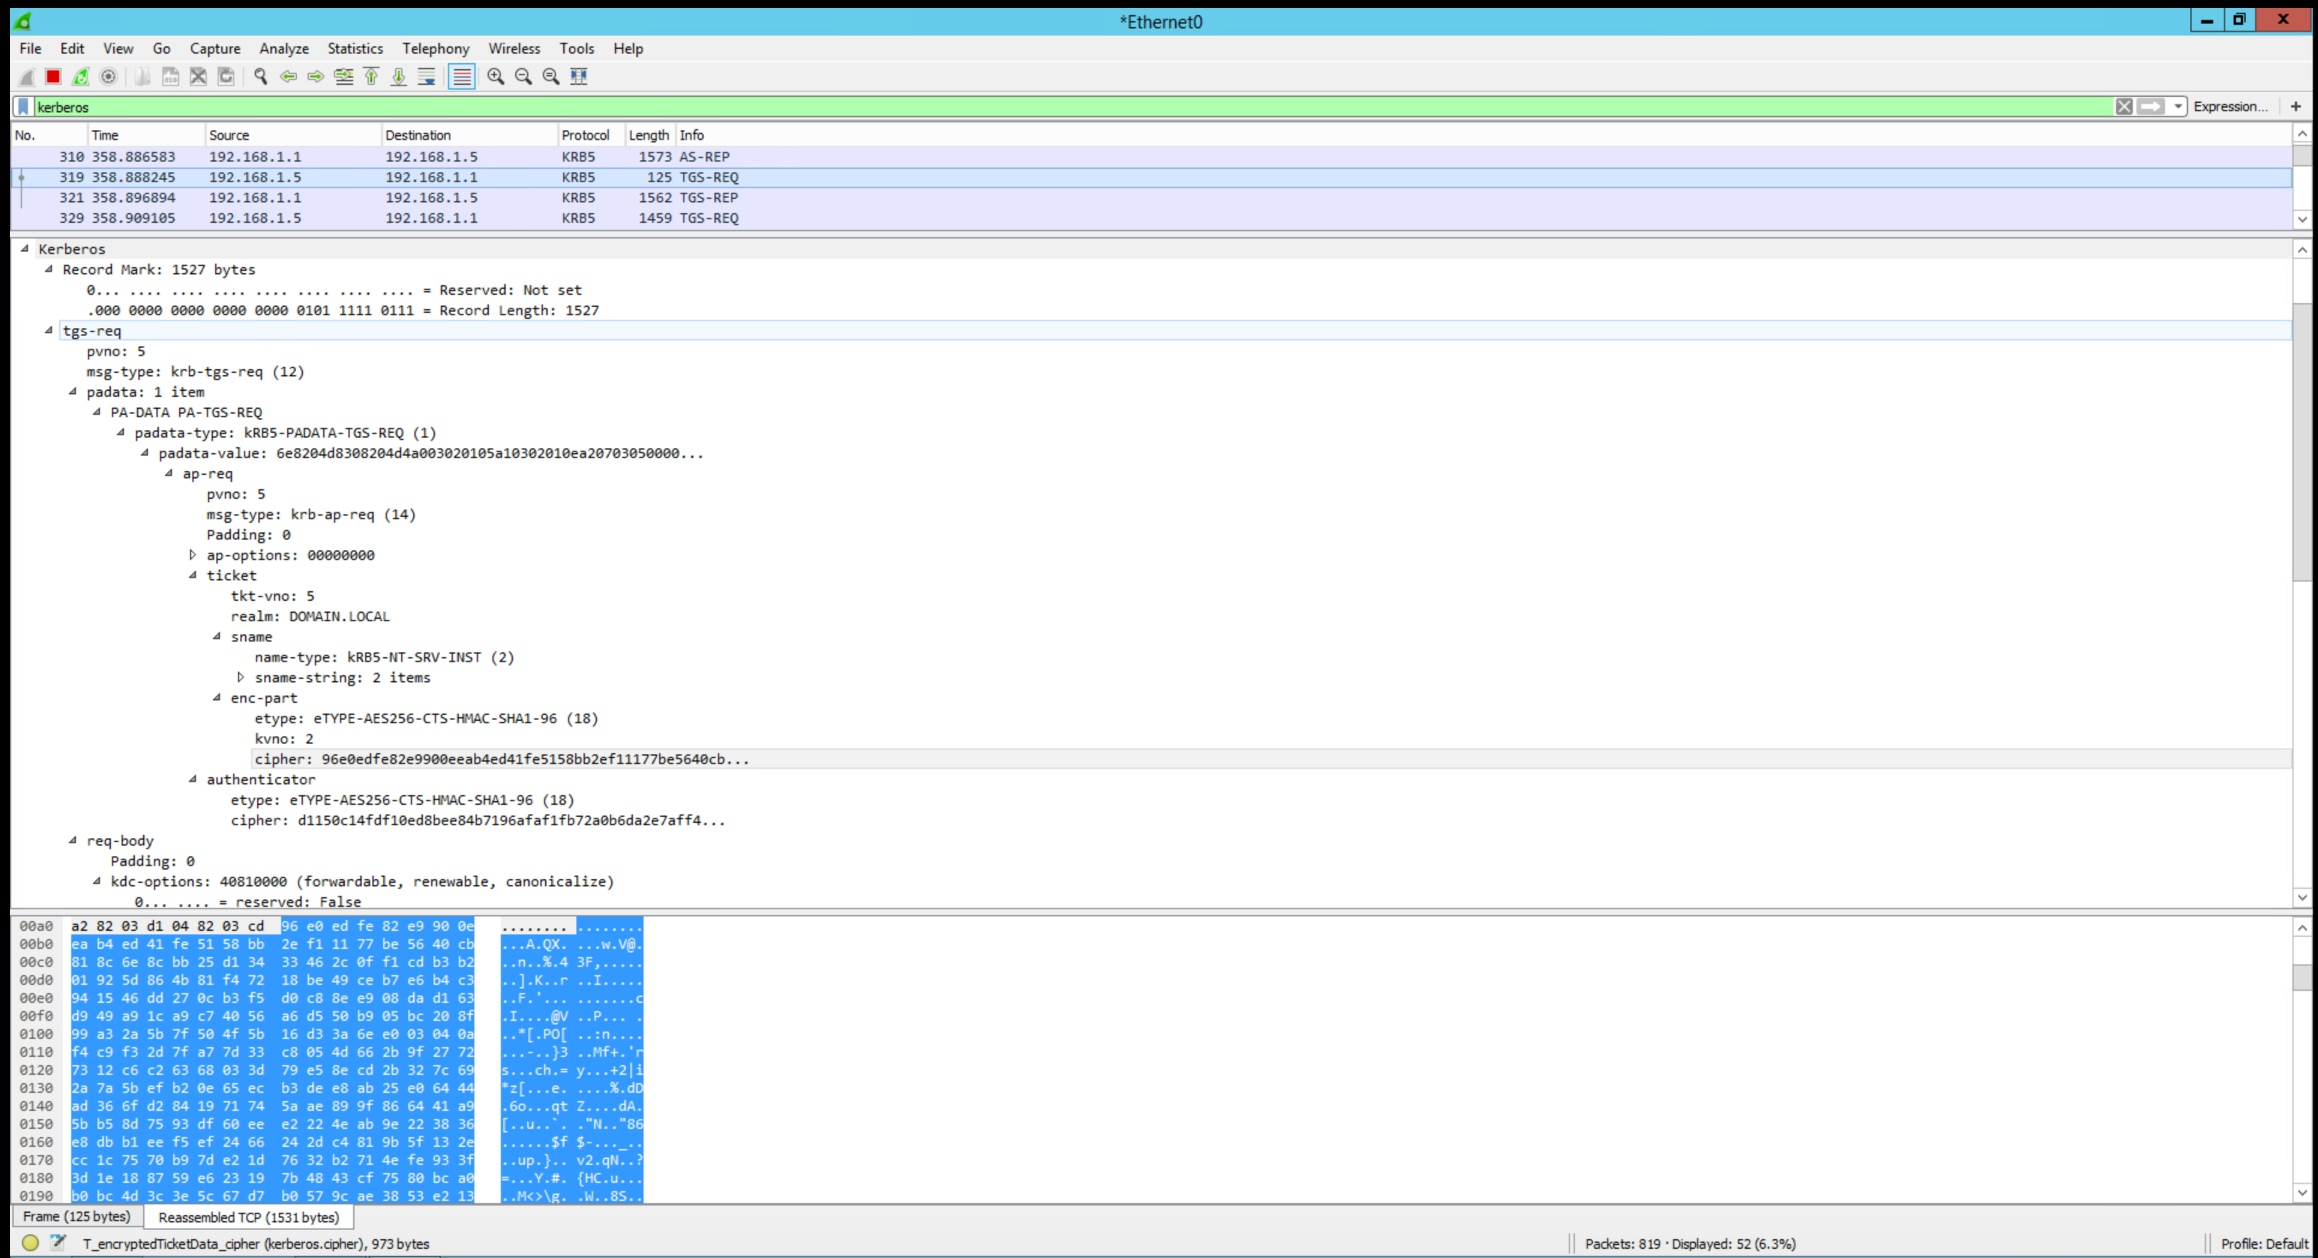
\includegraphics[scale=0.22]{pics/TGS-REQ.jpg}
    \end{center}
    TGS-REP:
    \vspace{-2em}
    \begin{center}
        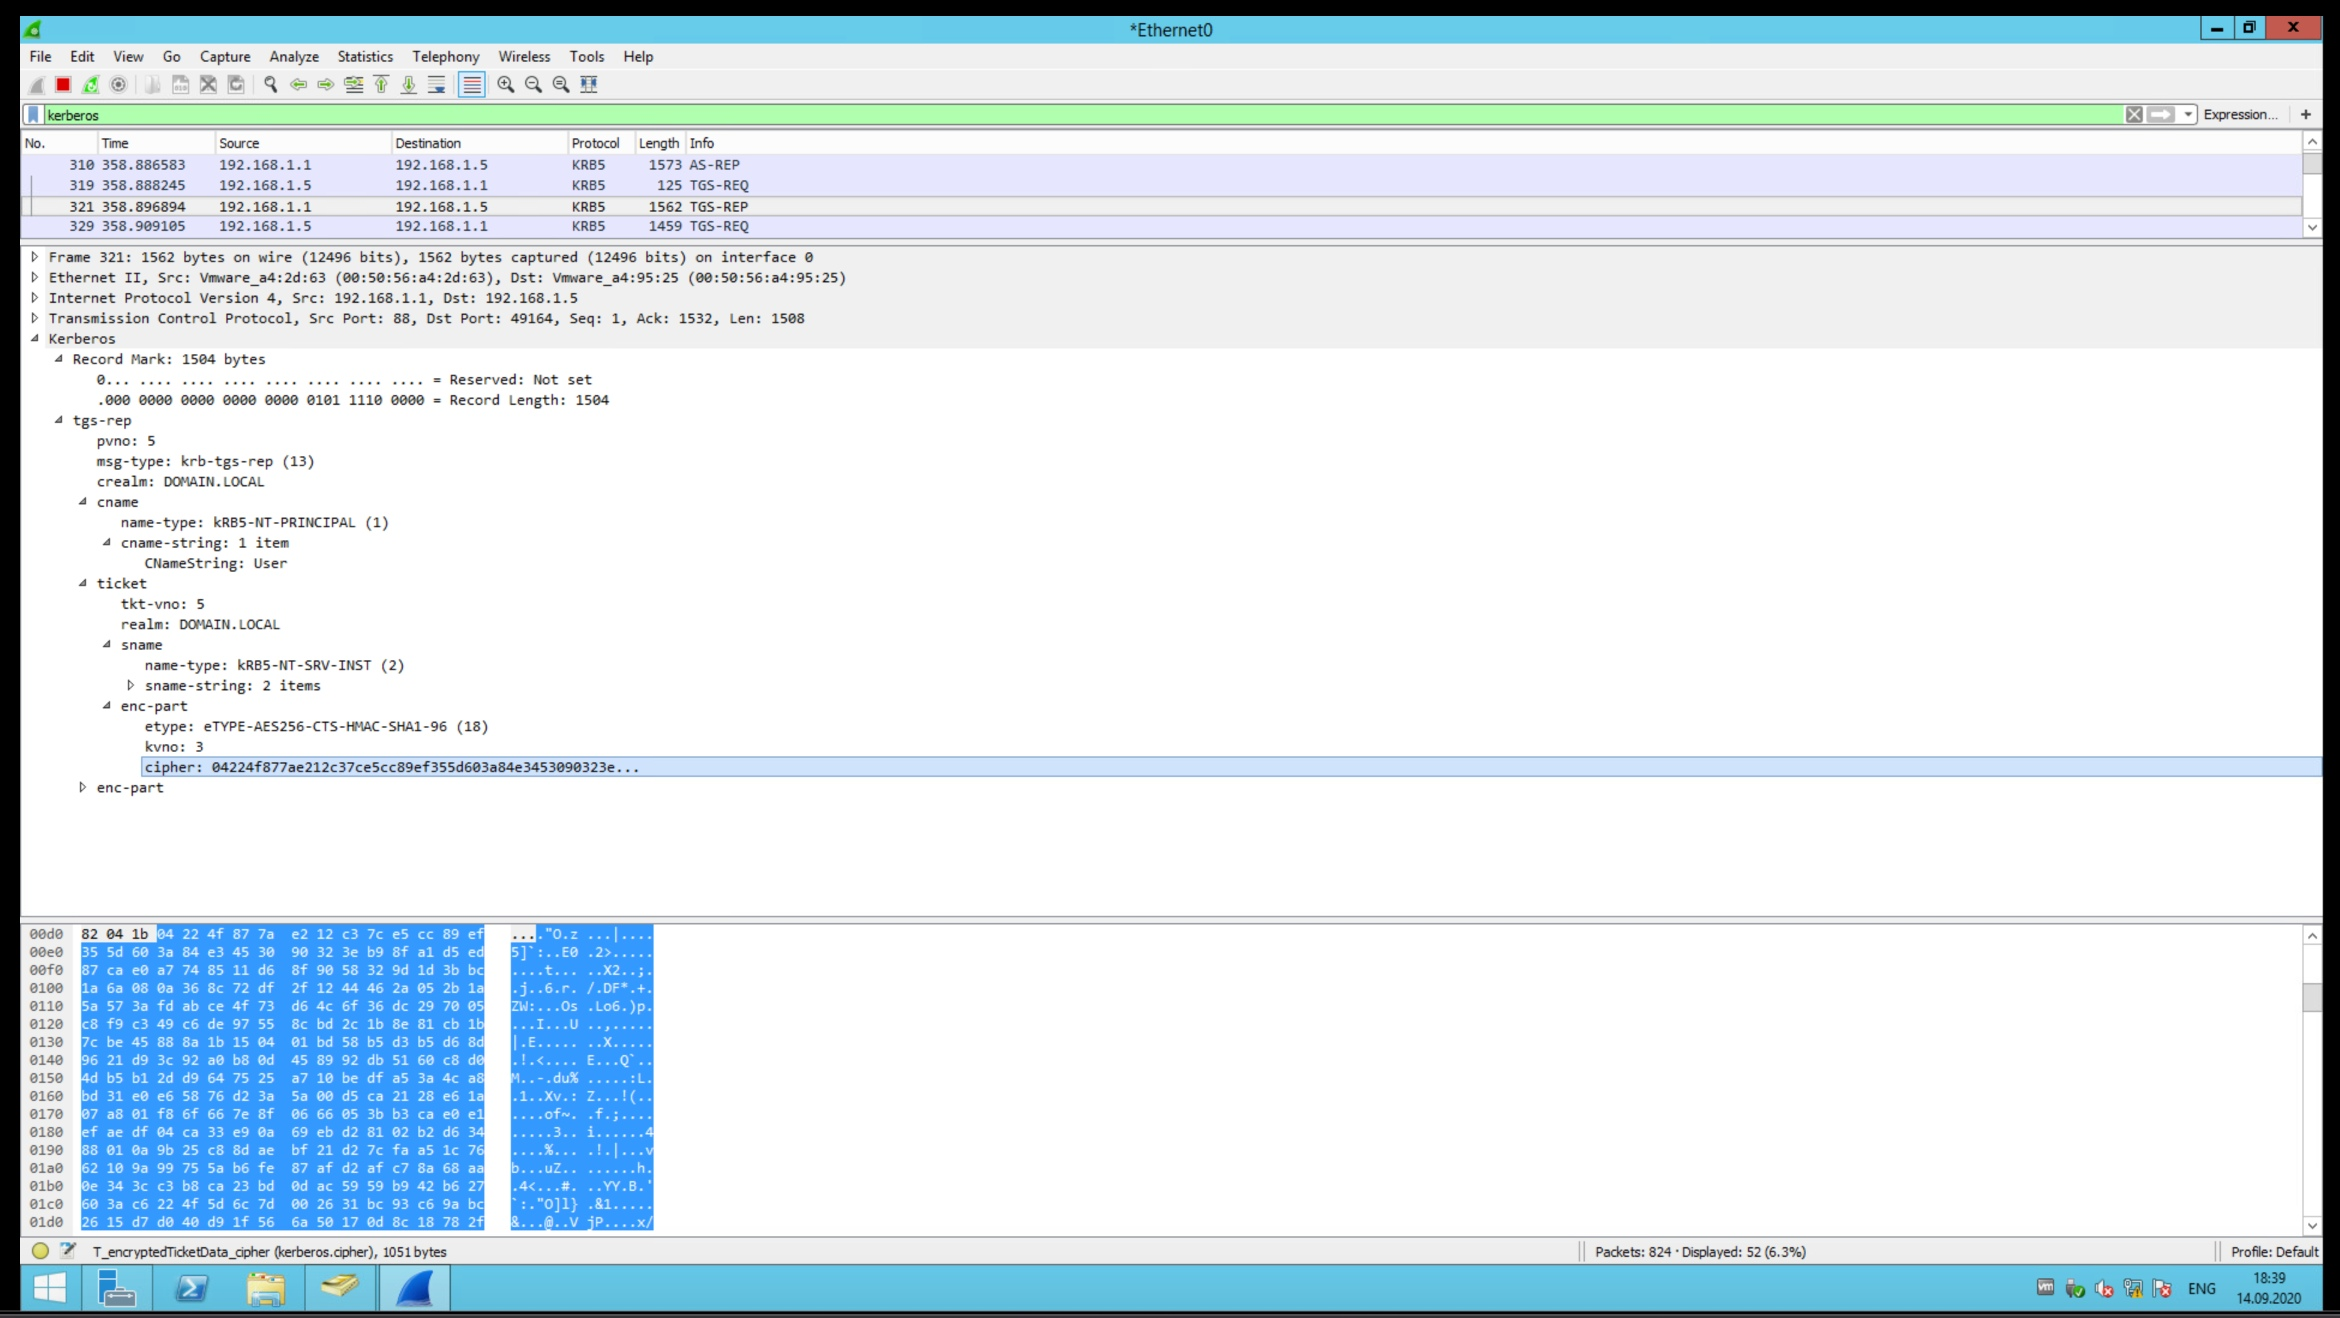
\includegraphics[scale=0.22]{pics/TGS-REP.jpg}
    \end{center}
    \newpage
    \textbf{Выводы}

    По итогам этой лабораторной работы, мы научились настраивать контрольный 
    домен и давать защищенный доступ клиентам к серверу. С помощью 
    программы Wireshark, мы разобрались в алгоритмах работы протоколов 
    Kerberos и NTLMv2. На скриншотах данной программы видно, как 
    компьютер-клиент безуспешно совершил 3 попытки отправки пакета 
    аутентификации NTLMv2 со стандартными логин/паролем, прежде чем запросил 
    у пользователя логин/пароль к серверу. 
    
\end{document}